\documentclass[10pt]{article}
\usepackage[a4paper,margin=18mm]{geometry}
\usepackage{amsmath,amssymb,booktabs,array,enumitem,longtable}
\usepackage[T1]{fontenc}\usepackage{lmodern}
\usepackage{tikz}\usetikzlibrary{shapes.gates.logic.US,positioning,arrows.meta,patterns,calc}
\usepackage[hidelinks]{hyperref}
\setlength{\parindent}{0pt}\setlength{\parskip}{4pt}\setlength{\emergencystretch}{2em}
\newcommand{\VDD}{V_{DD}}
\newcommand{\mos}[4]{\begin{scope}[shift={(#1,#2)}]
\draw (0,.24)--(0,-.24);\draw (0,.20)--(.25,.20)--(.25,.5);
\draw (0,-.20)--(.25,-.20)--(.25,-.5);\draw (-.16,.23)--(-.16,-.23);
\ifnum#4=1\draw (-.26,0) circle (.06);\draw (-.75,0)--(-.32,0);\else\draw (-.75,0)--(-.16,0);\fi
\node[anchor=east,font=\scriptsize] at (-.76,0) {$#3$};\end{scope}}
\newcommand{\ground}[2]{\draw (#1,#2)--(#1,{#2-.12});\draw ({#1-.17},{#2-.12})--({#1+.17},{#2-.12});\draw ({#1-.11},{#2-.20})--({#1+.11},{#2-.20});}
\newcommand{\rail}[3]{\draw (#1,#2)--(#1,{#2+.14});\node[above,font=\scriptsize] at (#1,{#2+.14}) {$#3$};}
\newcommand{\hmos}[4]{\begin{scope}[shift={(#1,#2)}]
\draw(-.24,0)--(.24,0);\draw(-.2,0)--(-.2,-.25)--(-.5,-.25);\draw(.2,0)--(.2,-.25)--(.5,-.25);
\draw(-.23,.16)--(.23,.16);
\ifnum#4=1\draw(0,.26)circle(.06);\draw(0,.32)--(0,.75);\else\draw(0,.16)--(0,.75);\fi
\node[below,font=\scriptsize]at(0,-.32){#3};\end{scope}}
\newcommand{\qheading}[1]{\par\medskip\textbf{#1}\par}
\begin{document}
\begin{center}{\large\bfseries EE3032 Introduction to VLSI Design---Final}\par Fall 2023\end{center}
\small Reconstruction from the two original printed pages; vector figures retain connectivity. The original point values sum to 115.\normalsize\par
\textbf{1. (30 points)} Answer the following questions.
\begin{enumerate}[label=(\alph*),leftmargin=7mm,itemsep=3pt]
\item List the components of dynamic power consumption of a dynamic logic gate. (6 points)
\item What is physical design? (2 points)
\item List two requirements for drawing the layout of a cell in the standard cell library. (4 points)
\item List two design methods for avoiding glitch power of a CMOS circuit. (4 points)
\item List two limitations of the dynamic logic. (4 points)
\item What is the goal of the design rule? (2 points)
\item Explain the function of filler cell, tap cell, decap cell, and endcap. (4 points)
\item Illustrate two possible technologies which can be used to shorten manufacturing time such that the time to market can be shortened. (4 points)
\end{enumerate}\textbf{2. (15 points)} Fig. 1(a) shows a domino logic circuit and the corresponding clock timing diagram. Complete the following questions.
\begin{enumerate}[label=(\alph*),leftmargin=7mm,itemsep=3pt]
\item If the output rise/fall times of the 3-input and 2-input AND gates are 3 ns/1 ns and 2 ns/1 ns, respectively, calculate the maximal operation frequency of the circuit. (5 points)
\item The clock period of this circuit cannot be prolonged casually. Why? Modify the circuit such that its clock period can be prolonged casually. Draw the transistor schematic diagram. (5 points)
\item Let the delay of each AND gate be 1 delay unit. If we apply the two input patterns (ABCD)=(0000,1110) in sequence, draw the output waveform with respect to input patterns. (5 points)
\end{enumerate}\begin{center}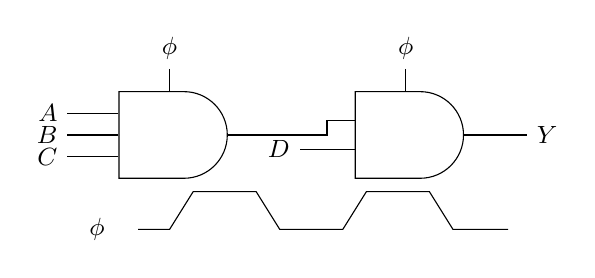
\begin{tikzpicture}[x=1cm,y=.8cm,font=\small]
\node[and gate US,draw,logic gate inputs=nnn,minimum width=1.1cm,minimum height=1.1cm] (a) at (0,1.5) {};
\node[and gate US,draw,logic gate inputs=nn,minimum width=1.1cm,minimum height=1.1cm] (b) at (3,1.5) {};
\foreach \n/\l in {1/A,2/B,3/C}{\draw(a.input \n)--++(-.65,0)node[left]{$\l$};}
\draw(a.output)--(2,1.5)|-(b.input 1);\draw(b.input 2)--++(-.7,0)node[left]{$D$};
\draw(b.output)--++(.8,0)node[right]{$Y$};
\draw(0,2.55)--(0,2.2)node[above,pos=0]{$\phi$};\draw(3,2.55)--(3,2.2)node[above,pos=0]{$\phi$};
\node[left]at(-.7,0){$\phi$};\draw(-.4,0)--(0,0)--(.3,.6)--(1.1,.6)--(1.4,0)--(2.2,0)--(2.5,.6)--(3.3,.6)--(3.6,0)--(4.3,0);
\end{tikzpicture}\end{center}
\begin{center}\small Figure 1(a): A domino logic circuit and its clock waveform.\end{center}\newpage\textbf{3. (10 points)} Fig. 1(b) shows a simple circuit with three gates. Complete the following questions.
\begin{enumerate}[label=(\alph*),leftmargin=7mm,itemsep=3pt]
\item Can the circuit be operated correctly? Explain your answer. If your answer is ``no'', modify the circuit such that it can be operated correctly. (5 points)
\item Assume that each transistor of the (modified) circuit has the following drain and gate capacitance: $C_d=0.1\,\mathrm{fF}$; $C_g=1\,\mathrm{fF}$; and the parasitic capacitance of the node $x$ and $y$ are $1.3\,\mathrm{fF}$ and $1.1\,\mathrm{fF}$, respectively. Let the switching voltage of all the gates in the (modified) circuit be $V_{DD}/2$. Can the circuit be operated correctly? Explain your answer. (5 points)
\end{enumerate}\begin{center}\begin{tikzpicture}[scale=.9,font=\small]
\mos{2}{4}{\phi}{1}\rail{2.25}{4.5}{V_{DD}}
\draw(.25,3.5)--(3.25,3.5);\fill(2.25,3.5)circle(1.5pt);
\mos{0}{3}{A}{0}\mos{0}{2}{B}{0}\mos{3}{3}{C}{0}\mos{2}{2}{A}{0}\mos{4}{2}{B}{0}
\draw(2.25,2.5)--(4.25,2.5);\fill(3.25,2.5)circle(1.5pt);\node[above]at(3.7,2.5){$y$};\node[right]at(.25,2.5){$x$};
\draw(.25,1.5)--(4.25,1.5);\mos{2}{1}{\phi}{0}\ground{2.25}{.5}
\mos{7}{3.8}{\bar\phi}{1}\rail{7.25}{4.3}{V_{DD}}\mos{7}{2.5}{}{0}
\draw(7.25,3)--(7.25,3.3);\draw(7.25,3.15)--(8.25,3.15)node[right]{$\overline Y$};
\mos{7}{1.5}{\bar\phi}{0}\ground{7.25}{1}
\mos{10}{4}{}{1}\node[above,font=\scriptsize]at(9.55,4.05){$\bar\phi$};\rail{10.25}{4.5}{V_{DD}}\mos{10}{3}{}{1}\mos{10}{1.8}{\bar\phi}{0}
\draw(10.25,2.3)--(10.25,2.5)--(11.1,2.5)node[right]{$X$};\ground{10.25}{1.3}
\draw(2.25,3.5)--(5.75,3.5)--(5.75,4.9)--(9,4.9)--(9,3)--(9.25,3);
\draw(5.75,3.5)--(5.75,2.5)--(6.25,2.5);\fill(5.75,3.5)circle(1.5pt);
\end{tikzpicture}\end{center}
\begin{center}\small Figure 1(b): A simple circuit. The middle clock is transcribed as $\bar\phi$; its stroke touches the gate wire in the scan, so the solution also considers a $\phi$ reading.\end{center}\textbf{4. (15 points)} Design $f=\overline{x_1x_2+x_3}$ using (1) dynamic logic and (2) differential pass transistor logic; design
\[
f=x_1\oplus x_2=\overline{x_1x_2+\overline{x_1+x_2}}
\]
using (3) NP domino logic.\newpage\textbf{5. (15 points)} Fig. 2(a) shows a Schmitt trigger circuit. If we apply an input signal as shown in the left figure to the Schmitt trigger circuit, the output signal will be as the right figure shows. Assume that $\mu_n=2\mu_p$; the drain parasitic capacitance of all the transistors can be ignored; and the simple RC delay model is used to estimate the delay. Complete the following questions.
\begin{enumerate}[label=(\alph*),leftmargin=7mm,itemsep=3pt]
\item Let $V_{tn}=|V_{tp}|=0.2\,\mathrm V$ and $V_{DD}=1.5\,\mathrm V$. If the size of N1 is $160\,\mathrm{nm}/40\,\mathrm{nm}$, determine the sizes of the transistors N2, N3, P1, P2, and P3 such that $t_r=t_f=3RC$, where the turn-on resistance and gate capacitance of N1 is $R$ and $C$. All the transistors should have the same channel length. (5 points)
\item Fig. 2(b) shows a Schmitt trigger circuit (STC) with controllable hysteresis voltage ($V_H$) by controlling the switches (sw). If the switches are turned on, is the noise tolerance capability of the STC increased or decreased? Is the short-circuit power of STC increased or decreased? Explain your answers. (10 points)
\end{enumerate}\begin{center}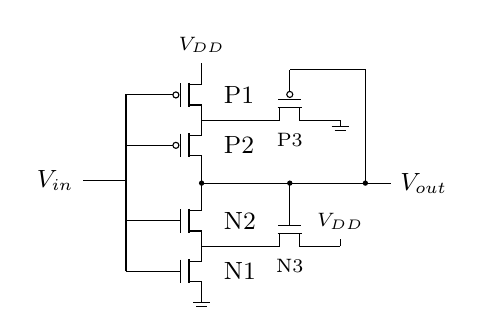
\begin{tikzpicture}[scale=0.64,font=\small]
\mos{1}{5}{}{1}\mos{1}{4}{}{1}\mos{1}{2.5}{}{0}\mos{1}{1.5}{}{0}
\rail{1.25}{5.5}{V_{DD}}\ground{1.25}{1}\draw(1.25,3)--(1.25,3.5);\draw(1.25,3.25)--(5.0,3.25)node[right]{$V_{out}$};\fill(1.25,3.25)circle(1.5pt);
\draw(-.25,1.5)--(-.25,5)--(.25,5);\draw(-.25,4)--(.25,4);\draw(-.25,2.5)--(.25,2.5);\draw(-.25,1.5)--(.25,1.5);\draw(-1.1,3.3)--(-.25,3.3)node[pos=0,left]{$V_{in}$};
\node[right]at(1.5,5){P1};\node[right]at(1.5,4){P2};\node[right]at(1.5,2.5){N2};\node[right]at(1.5,1.5){N1};
\hmos{3}{4.75}{P3}{1}\draw(1.25,4.5)--(2.5,4.5);\draw(3.5,4.5)--(4,4.5);\ground{4}{4.5}
\hmos{3}{2.25}{N3}{0}\draw(1.25,2)--(2.5,2);\draw(3.5,2)--(4,2);\rail{4}{2}{V_{DD}}
\draw(3,3)--(3,3.25);\fill(3,3.25)circle(1.5pt);\draw(3,5.5)--(4.5,5.5)--(4.5,3.25);\fill(4.5,3.25)circle(1.5pt);
\end{tikzpicture}\qquad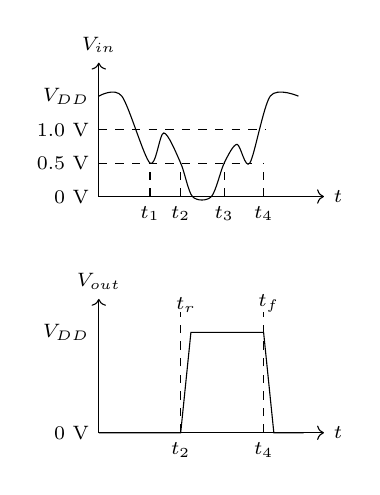
\begin{tikzpicture}[x=.65cm,y=.85cm,font=\scriptsize]
\draw[->](0,0)--(4.4,0)node[right]{$t$};\draw[->](0,0)--(0,2.0)node[above]{$V_{in}$};
\draw plot[smooth]coordinates{(0,1.5)(.45,1.5)(1,.5)(1.27,.95)(1.6,.5)(1.83,0)(2.2,0)(2.45,.5)(2.7,.78)(2.95,.5)(3.35,1.5)(3.9,1.5)};
\draw[dashed](0,1)--(3.25,1);\draw[dashed](0,.5)--(3.0,.5);\node[left]at(0,1.5){$V_{DD}$};\node[left]at(0,1){1.0 V};\node[left]at(0,.5){0.5 V};\node[left]at(0,0){0 V};
\foreach\x/\l in {1/1,1.6/2,2.45/3,3.22/4}{\draw[dashed](\x,0)--(\x,.5);\node[below]at(\x,0){$t_\l$};}
\begin{scope}[yshift=-3cm]
\draw[->](0,0)--(4.4,0)node[right]{$t$};\draw[->](0,0)--(0,2)node[above]{$V_{out}$};\node[left]at(0,1.5){$V_{DD}$};\node[left]at(0,0){0 V};
\draw(0,0)--(1.6,0)--(1.8,1.5)--(3.22,1.5)--(3.42,0)--(4.0,0);\draw[dashed](1.6,0)--(1.6,1.8);\draw[dashed](3.22,0)--(3.22,1.8);\node[above]at(1.7,1.65){$t_r$};\node[above]at(3.32,1.65){$t_f$};\node[below]at(1.6,0){$t_2$};\node[below]at(3.22,0){$t_4$};
\end{scope}\end{tikzpicture}\par (a)\end{center}
\begin{center}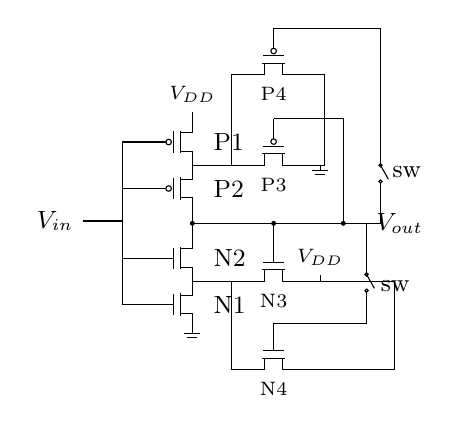
\begin{tikzpicture}[scale=0.59,font=\small]
\mos{1}{5}{}{1}\mos{1}{4}{}{1}\mos{1}{2.5}{}{0}\mos{1}{1.5}{}{0}
\rail{1.25}{5.5}{V_{DD}}\ground{1.25}{1}\draw(1.25,3)--(1.25,3.5);\draw(1.25,3.25)--(5.0,3.25)node[right]{$V_{out}$};\fill(1.25,3.25)circle(1.5pt);
\draw(-.25,1.5)--(-.25,5)--(.25,5);\draw(-.25,4)--(.25,4);\draw(-.25,2.5)--(.25,2.5);\draw(-.25,1.5)--(.25,1.5);\draw(-1.1,3.3)--(-.25,3.3)node[pos=0,left]{$V_{in}$};
\node[right]at(1.5,5){P1};\node[right]at(1.5,4){P2};\node[right]at(1.5,2.5){N2};\node[right]at(1.5,1.5){N1};
\hmos{3}{4.75}{P3}{1}\draw(1.25,4.5)--(2.5,4.5);\draw(3.5,4.5)--(4,4.5);\ground{4}{4.5}
\hmos{3}{2.25}{N3}{0}\draw(1.25,2)--(2.5,2);\draw(3.5,2)--(4,2);\rail{4}{2}{V_{DD}}
\draw(3,3)--(3,3.25);\fill(3,3.25)circle(1.5pt);\draw(3,5.5)--(4.5,5.5)--(4.5,3.25);\fill(4.5,3.25)circle(1.5pt);
\hmos{3}{6.7}{P4}{1}\draw(1.25,4.5)--(2.1,4.5)--(2.1,6.45)--(2.5,6.45);\draw(3.5,6.45)--(4.1,6.45)--(4.1,4.5)--(4,4.5);
\hmos{3}{.35}{N4}{0}\draw(1.25,2)--(2.1,2)--(2.1,.1)--(2.5,.1);\draw(3.5,.1)--(5.6,.1)--(5.6,2)--(4,2);
\draw(3,7.45)--(5.3,7.45)--(5.3,4.5);\draw(5.3,4.15)--(5.3,3.25)--(4.5,3.25);\draw(5.3,4.5)--(5.47,4.2);\draw(5.3,4.5)circle(.035);\draw(5.3,4.15)circle(.035);\node[right]at(5.35,4.35){sw};
\draw(3,1.1)--(5.0,1.1)--(5.0,1.8);\draw(5.0,2.15)--(5.0,3.25);\draw(5.0,2.15)--(5.17,1.85);\draw(5.0,1.8)circle(.035);\draw(5.0,2.15)circle(.035);\node[right]at(5.1,1.9){sw};
\end{tikzpicture}\par (b)\end{center}
\begin{center}\small Figure 2: (a) A CMOS Schmitt trigger circuit (b) A STC with controllable hysteresis voltage.\end{center}
\newpage\textbf{6. (10 points)} Draw the transistor-level schematic diagram of the symbolic layout shown in Fig. 3(a).
% Normalized topological geometry: 7 crossings/row, 14physical MOS.
\usetikzlibrary{patterns}
\begin{center}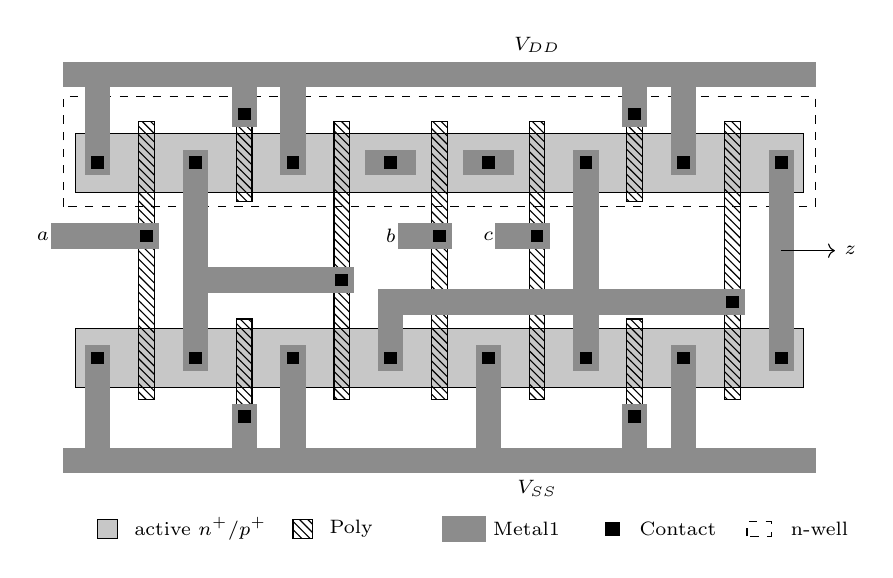
\begin{tikzpicture}[x=.62cm,y=.62cm,font=\scriptsize]
\tikzset{mone/.style={draw=black!45,line width=.32cm,line cap=rect},poly/.style={draw,pattern=north west lines}}
% Continuous active diffusion strips and upper n-well.
\filldraw[fill=black!22](-.45,4) rectangle(14.45,5.2);
\filldraw[fill=black!22](-.45,0) rectangle(14.45,1.2);
\draw[dashed](-.7,3.7)rectangle(14.7,5.95);
% Functional polys: a, x, b, c, w. Two split isolation columns: 2 and6.
\foreach \g in {1,5,7,9,13}{\filldraw[poly](\g-.16,-.25)rectangle(\g+.16,5.45);}
\foreach \g in {3,11}{\filldraw[poly](\g-.16,3.8)rectangle(\g+.16,5.65);\filldraw[poly](\g-.16,-.7)rectangle(\g+.16,1.4);}
% Metal1 rail distribution and contact branches.
\draw[mone](-.45,6.4)--(14.45,6.4);\node[above]at(9,6.65){$V_{DD}$};
\draw[mone](-.45,-1.5)--(14.45,-1.5);\node[below]at(9,-1.7){$V_{SS}$};
\foreach \x in {0,4,12}{\draw[mone](\x,4.6)--(\x,6.4);\fill(\x-.13,4.47)rectangle(\x+.13,4.73);}
\foreach \x in {0,4,8,12}{\draw[mone](\x,.6)--(\x,-1.5);\fill(\x-.13,.47)rectangle(\x+.13,.73);}
% Left inverter drain strap x, feeding column3 via metal/poly contact.
\draw[mone](2,.6)--(2,4.6);\fill(1.87,.47)rectangle(2.13,.73);\fill(1.87,4.47)rectangle(2.13,4.73);
\draw[mone](2,2.2)--(5,2.2);\fill(4.87,2.07)rectangle(5.13,2.33);
% Series-PMOS internal local contact/metal patches: p1,p2, not supply.
\foreach \x/\n in {6/p_1,8/p_2}{\draw[mone](\x-.27,4.6)--(\x+.27,4.6);\fill(\x-.13,4.47)rectangle(\x+.13,4.73);}
% w joins PMOS segment5/6, NMOS3/4 and5/6, then drives column7.
\draw[mone](10,.6)--(10,4.6);\fill(9.87,.47)rectangle(10.13,.73);\fill(9.87,4.47)rectangle(10.13,4.73);
\draw[mone](6,.6)--(6,1.75)--(13,1.75);\draw[mone](10,1.75)--(13,1.75);
\fill(5.87,.47)rectangle(6.13,.73);\fill(12.87,1.62)rectangle(13.13,1.88);
% Right inverter drain strap, labeled output z.
\draw[mone](14,.6)--(14,4.6);\fill(13.87,.47)rectangle(14.13,.73);\fill(13.87,4.47)rectangle(14.13,4.73);
\draw[->](14,2.8)--(15.1,2.8)node[right]{$z$};
% Input metal/poly contacts; rail-tied isolation gate stubs.
\draw[mone](-.7,3.1)--(1,3.1);\fill(.87,2.97)rectangle(1.13,3.23);\node[left]at(-.8,3.1){$a$};
\draw[mone](6.4,3.1)--(7,3.1);\fill(6.87,2.97)rectangle(7.13,3.23);\node[left]at(6.3,3.1){$b$};
\draw[mone](8.4,3.1)--(9,3.1);\fill(8.87,2.97)rectangle(9.13,3.23);\node[left]at(8.3,3.1){$c$};
\foreach \g in {3,11}{\draw[mone](\g,5.6)--(\g,6.4);\fill(\g-.13,5.47)rectangle(\g+.13,5.73);\draw[mone](\g,-.6)--(\g,-1.5);\fill(\g-.13,-.73)rectangle(\g+.13,-.47);}
% Layer legend. A crossing without a black contact square is insulated.
\filldraw[fill=black!22](0,-3.1)rectangle(.4,-2.7);\node[right]at(.55,-2.9){active $n^+/p^+$};
\filldraw[poly](4,-3.1)rectangle(4.4,-2.7);\node[right]at(4.55,-2.9){Poly};
\draw[mone](7.3,-2.9)--(7.7,-2.9);\node[right]at(7.9,-2.9){Metal1};
\fill(10.4,-3.05)rectangle(10.7,-2.75);\node[right]at(10.9,-2.9){Contact};
\draw[dashed](13.3,-3.05)rectangle(13.8,-2.75);\node[right]at(14,-2.9){n-well};
\end{tikzpicture}\end{center}
\begin{center}\small Figure 3(a): Symbolic layout. Normalized geometry preserves all contacts and all seven poly crossings per active row; scale is not specified in the original.\end{center}\begin{center}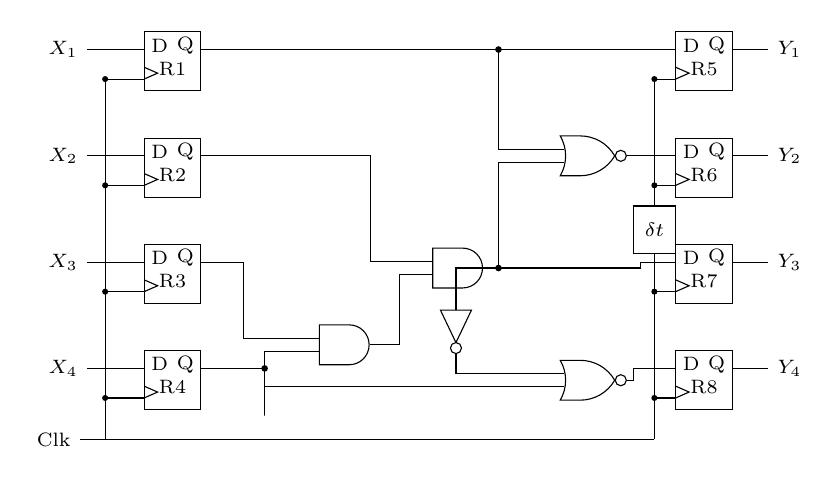
\begin{tikzpicture}[x=.9cm,y=.75cm,font=\scriptsize]
\draw(0.29999999999999993,6.5)rectangle(1.1,7.5);\node at(0.7,6.88){R1};
\node at(0.52,7.27){D};\node at(0.8799999999999999,7.27){Q};
\draw(0.29999999999999993,6.7)--(0.49,6.8)--(0.29999999999999993,6.9);
\draw(7.799999999999999,6.5)rectangle(8.6,7.5);\node at(8.2,6.88){R5};
\node at(8.02,7.27){D};\node at(8.379999999999999,7.27){Q};
\draw(7.799999999999999,6.7)--(7.989999999999999,6.8)--(7.799999999999999,6.9);
\draw(-.5,7.2)--(.3,7.2)node[pos=0,left]{$X_1$};
\draw(8.6,7.2)--(9.1,7.2)node[right]{$Y_1$};
\draw(0.29999999999999993,4.7)rectangle(1.1,5.7);\node at(0.7,5.08){R2};
\node at(0.52,5.470000000000001){D};\node at(0.8799999999999999,5.470000000000001){Q};
\draw(0.29999999999999993,4.9)--(0.49,5.0)--(0.29999999999999993,5.1000000000000005);
\draw(7.799999999999999,4.7)rectangle(8.6,5.7);\node at(8.2,5.08){R6};
\node at(8.02,5.470000000000001){D};\node at(8.379999999999999,5.470000000000001){Q};
\draw(7.799999999999999,4.9)--(7.989999999999999,5.0)--(7.799999999999999,5.1000000000000005);
\draw(-.5,5.4)--(.3,5.4)node[pos=0,left]{$X_2$};
\draw(8.6,5.4)--(9.1,5.4)node[right]{$Y_2$};
\draw(0.29999999999999993,2.9)rectangle(1.1,3.9);\node at(0.7,3.28){R3};
\node at(0.52,3.67){D};\node at(0.8799999999999999,3.67){Q};
\draw(0.29999999999999993,3.1)--(0.49,3.1999999999999997)--(0.29999999999999993,3.3);
\draw(7.799999999999999,2.9)rectangle(8.6,3.9);\node at(8.2,3.28){R7};
\node at(8.02,3.67){D};\node at(8.379999999999999,3.67){Q};
\draw(7.799999999999999,3.1)--(7.989999999999999,3.1999999999999997)--(7.799999999999999,3.3);
\draw(-.5,3.6)--(.3,3.6)node[pos=0,left]{$X_3$};
\draw(8.6,3.6)--(9.1,3.6)node[right]{$Y_3$};
\draw(0.29999999999999993,1.0999999999999996)rectangle(1.1,2.0999999999999996);\node at(0.7,1.4799999999999995){R4};
\node at(0.52,1.8699999999999997){D};\node at(0.8799999999999999,1.8699999999999997){Q};
\draw(0.29999999999999993,1.2999999999999996)--(0.49,1.3999999999999997)--(0.29999999999999993,1.4999999999999996);
\draw(7.799999999999999,1.0999999999999996)rectangle(8.6,2.0999999999999996);\node at(8.2,1.4799999999999995){R8};
\node at(8.02,1.8699999999999997){D};\node at(8.379999999999999,1.8699999999999997){Q};
\draw(7.799999999999999,1.2999999999999996)--(7.989999999999999,1.3999999999999997)--(7.799999999999999,1.4999999999999996);
\draw(-.5,1.7999999999999996)--(.3,1.7999999999999996)node[pos=0,left]{$X_4$};
\draw(8.6,1.7999999999999996)--(9.1,1.7999999999999996)node[right]{$Y_4$};
\node[and gate US,draw,logic gate inputs=nn] (a1) at(3.1,2.2) {};
\node[and gate US,draw,logic gate inputs=nn] (a2) at(4.7,3.5) {};
\node[nor gate US,draw,logic gate inputs=nn] (n1) at(6.5,5.4) {};
\node[nor gate US,draw,logic gate inputs=nn] (n2) at(6.5,1.6) {};
\node[not gate US,draw,rotate=-90] (iv) at(4.7,2.6) {};
\draw(1.1,3.6)--(1.7,3.6)|-(a1.input 1);
\draw(1.1,1.8)--(2,1.8)|-(a1.input 2);
\draw(1.1,5.4)--(3.5,5.4)|-(a2.input 1);\draw(a1.output)--(3.9,2.2)|-(a2.input 2);
\draw(a2.output)--(5.3,3.5)--(7.3,3.5)|-(7.8,3.6);\fill(5.3,3.5)circle(1.2pt);
\draw(5.3,3.5)--(5.3,5.1)|-(n1.input 2);\draw(5.3,3.5)--(4.7,3.5)--(iv.input);
\draw(iv.output)--(4.7,1.8)|-(n2.input 1);
\draw(2,1.8)--(2,1)|-(n2.input 2);\fill(2,1.8)circle(1.2pt);
\draw(n1.output)--(7.8,5.4);\draw(n2.output)--(7.2,1.6)|-(7.8,1.8);
\draw(1.1,7.2)--(7.8,7.2);\draw(5.3,7.2)--(5.3,5.7)|-(n1.input 1);\fill(5.3,7.2)circle(1.2pt);
\draw(-.25,.6)--(-.25,6.7);\draw(-.6,.6)--(7.5,.6)node[pos=0,left]{Clk};
\draw(-.25,6.7)--(.3,6.7);\fill(-.25,6.7)circle(1.1pt);
\draw(7.5,6.7)--(7.8,6.7);\fill(7.5,6.7)circle(1.1pt);
\draw(-.25,4.9)--(.3,4.9);\fill(-.25,4.9)circle(1.1pt);
\draw(7.5,4.9)--(7.8,4.9);\fill(7.5,4.9)circle(1.1pt);
\draw(-.25,3.1)--(.3,3.1);\fill(-.25,3.1)circle(1.1pt);
\draw(7.5,3.1)--(7.8,3.1);\fill(7.5,3.1)circle(1.1pt);
\draw(-.25,1.3)--(.3,1.3);\fill(-.25,1.3)circle(1.1pt);
\draw(7.5,1.3)--(7.8,1.3);\fill(7.5,1.3)circle(1.1pt);
\draw(7.5,.6)--(7.5,3.75);\draw(7.5,4.55)--(7.5,6.7);
\draw(7.2,3.75)rectangle(7.8,4.55);\node at(7.5,4.15){$\delta t$};
\end{tikzpicture}\end{center}
\begin{center}\small Figure 3(b): A sequential circuit. The inline capture-clock delay is below R6 and above R7.\end{center}\textbf{7. (20 points)} Fig. 3(b) shows a sequential circuit. Assume that the clock-to-Q propagation delay ($t_{pcq}$), the clock-to-Q contamination delay ($t_{ccq}$), the setup time ($t_{setup}$), and the hold time ($t_{hold}$) of the registers are 0.2 ns, 0.1 ns, 0.2 ns, and 0.2 ns, respectively. The delay of the AND gate, the NOR gate, and the inverter is 0.5 ns, 0.5 ns, and 0.2 ns, respectively. Also, the delay of interconnection can be ignored. Complete the following questions.
\begin{enumerate}[label=(\alph*),leftmargin=7mm,itemsep=3pt]
\item Let $\delta t=0$ ns. Can the circuit be operated correctly? If not, modify the circuit by adding a lockup latch such that it can operate correctly and draw the modified circuit. (5 points)
\item Let $\delta t=0$ ns. Determine the maximum operation frequency of the circuit or the modified circuit. (5 points)
\item Let $\delta t=0.3$ ns. Can the circuit be operated correctly? If yes, is the maximum operation frequency of the circuit changed? Explain your answers. (5 points)
\item The registers typically are randomly distributed in a die. List two typical clock design methods for minimizing the clock skews among the registers. You should explain why the methods can minimize the clock skews. (5 points)
\end{enumerate}\end{document}